% definit le type de document et ses options
\documentclass[a4paper,10pt]{article}

% des paquetages indispensables, qui ajoutent des fonctionnalites

%\usepackage[cyr]{aeguill}
%\usepackage[francais]{babel}
\usepackage[utf8]{inputenc}
\usepackage[T1]{fontenc}
\usepackage{amsmath,amssymb}
\usepackage{fullpage}
\usepackage{graphicx}
\usepackage{latexsym}
\usepackage{here}
\usepackage{url}
\usepackage{ulem}
\usepackage{xspace}
\usepackage{picins}
\usepackage{geometry}
\usepackage{fancyhdr, color}


\title{\textbf{Rapport de TP : Optimisation Numérique}}
\author{Jean-Baptiste \bsc{Keck}, Gauthier \bsc{Zirnhelt} \\ \\ Groupe 1 - MMIS - 2A - \bsc{Ensimag}}

\date{\today}


\pagestyle{fancy}
\fancyhead[]{}
\renewcommand{\headrulewidth}{0pt}
\renewcommand\footrulewidth{1pt}
\fancyfoot[C]{   }
\fancyfoot[L]{\textbf{TP Optimisation Numérique} - Groupe 1 - MMIS - 2A - \bsc{Ensimag}}
\fancyfoot[R]{\textbf{Page \thepage}}

\geometry{scale=0.9, nohead}

\definecolor{lightgray}{gray}{0.9}

\newcommand*{\bigchi}{\mbox{\Large$\chi$}}% big chi
\newcommand*{\bige}{\mbox{\Large$\mathcal{E}$}}% bigexp 
\newcommand*\E{\ensuremath{\textup{e}}\xspace} %exponentielle
\newcommand{\II}{\mbox{\large 1\hskip -0,353em 1}} %échelon

%===============
\begin{document}
%===============


% pour afficher titre, auteur et date
\maketitle
\hrulefill

\\
\vspace{5cm}
\section{Analyse des méthodes à direction de descente}

\vspace{0.5cm}
\subsection{Avant propos}

\hspace{0.4cm}
Tous les algorithmes et les graphiques ont été réalisés en $\verb!C++!$ grâce aux librairies $blitz$, $gsl$ et $plplot$ afin de pouvoir mieux analyser leur exécution, notamment avec des outils de profiling.

\\
\vspace{0.5cm}
\noindent Les algorithmes étudiés dans ce rapport sont : 
\begin{itemize}
	\item L'algorithme du gradient à pas fixe
	\item L'algorithme du gradient avec recherche linéaire de Wolfe
	\item \sout{L'algorithme BFGS}*
	\item L'algorithme de Newton
	\item L'algorithme de Newton avec recherche linéaire de Wolfe
\end{itemize}

*Suite aux nombreuses tentatives de debug cet algorithme fait toujours tourner Wolfe dans une direction qui n'est pas une direction de descente et ne s'arrête pas.

\vspace{0.5cm}
\noindent Dans toute la suite on considère que le nombre maximal d'itérations autorisé est de $N = 10^6$ et que critère d'arrêt sur la norme euclidienne du gradient est de $\epsilon = 10^{-6}$. Le point initial est toujours $x_0$.


\newpage
\subsection{Fonctions étudiées}
\vspace{0.5cm}
\subsubsection{Première fonction}

\vspace{0.5cm}
\hspace{0.4cm}
C'est la fonction de base du TP. 

$$
f(x) = \sum_{k=1}^{n} kx_k^2
$$

\vspace{0.5cm}
Pour le tracé on se place dans le cas n = 2, $f(x,y) = x^2 + 2y^2$ avec $x_0 = (1.8,1.8)$.

\begin{figure}[H]
	\centering
	\subfloat{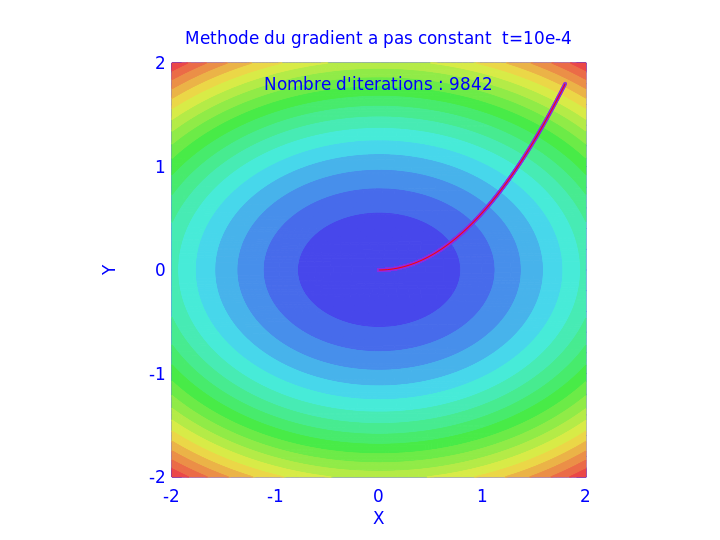
\includegraphics[width=9cm]{img/f_gradient.png}}
	\subfloat{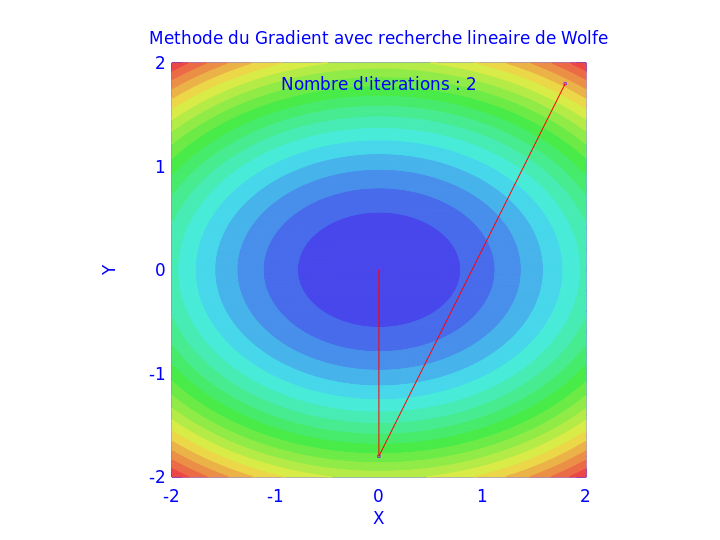
\includegraphics[width=9cm]{img/f_gradient_wolfe.png}}
\end{figure}

\begin{figure}[H]
	\centering
	\subfloat{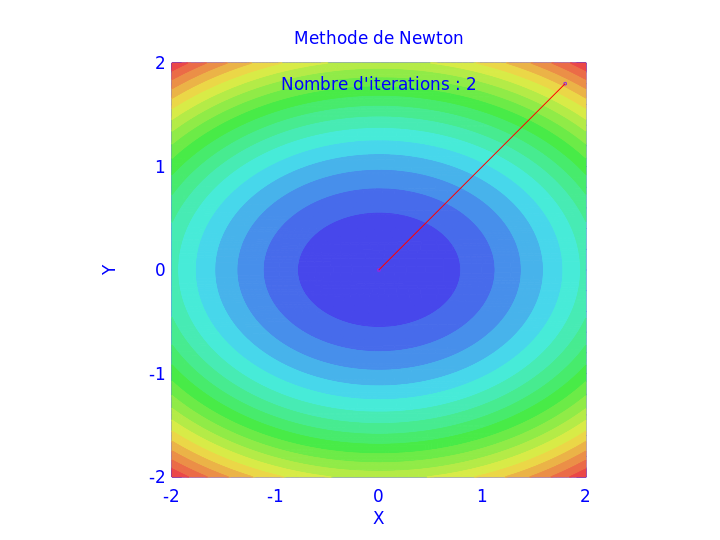
\includegraphics[width=9cm]{img/f_newton.png}}
	\subfloat{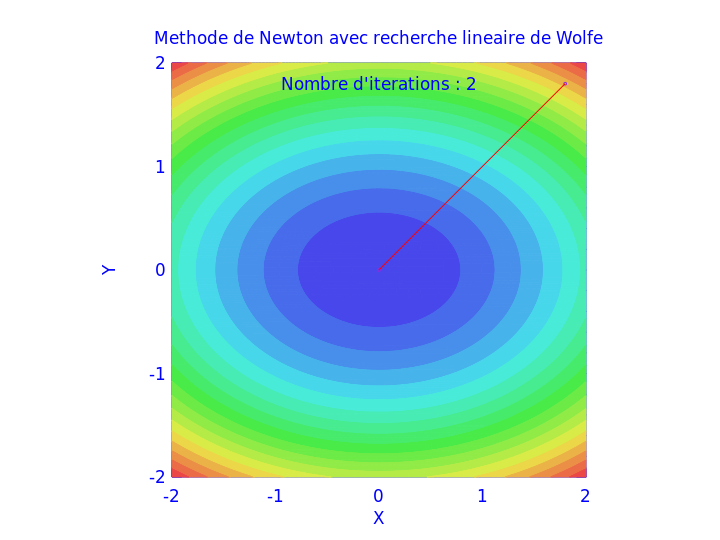
\includegraphics[width=9cm]{img/f_newton_wolfe.png}}
\end{figure}

\\
\vspace{0.5cm}
On constate que la methode de Newton à pas fixe met extrêmement longtemps à converger (presque 10 000 itérations) tandis que celle avec la recherche linéaire de Wolfe converge directement en deux itérations. Les méthodes de Newton convergent également directement.


\newpage
\subsubsection{Fonction de Rosenbrock}

\vspace{0.5cm}

\hspace{0.4cm}
Un peu plus intéressant pour tester nos algorithmes : la fonction de Rosenbrock.
Elle ne possède qu'un seul minimum 0 en $(1,1)$ mais n'est pas convexe comme la première fonction.
Le point initial considéré est $x_0 = (-0.2,1.2)$.

\begin{figure}[H]
	\centering
	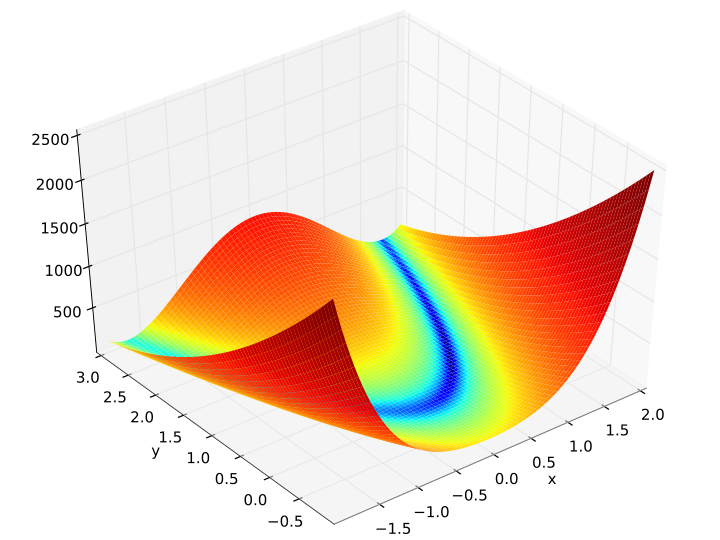
\includegraphics[width = 6cm]{img/rosenbrock.png}
\end{figure}

$$
f(x,y) = (1-x)^2 + 100(y-x^2)^2
$$

\begin{figure}[H]
	\centering
	\subfloat{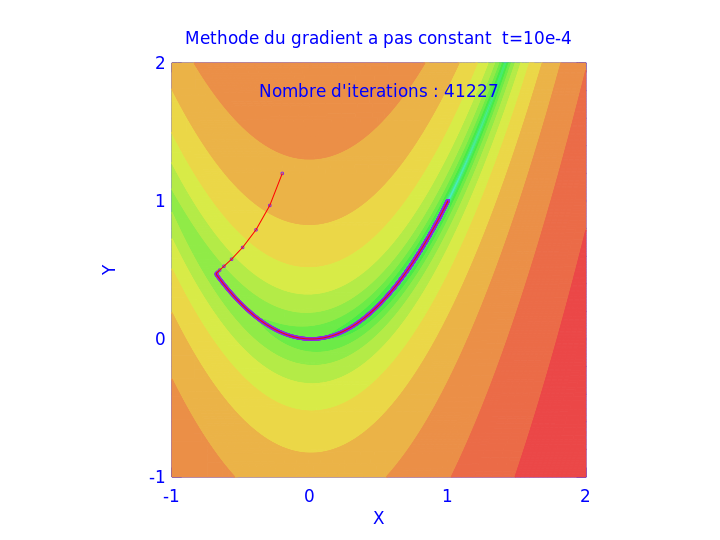
\includegraphics[width=9cm]{img/rosenbrock_gradient.png}}
	\subfloat{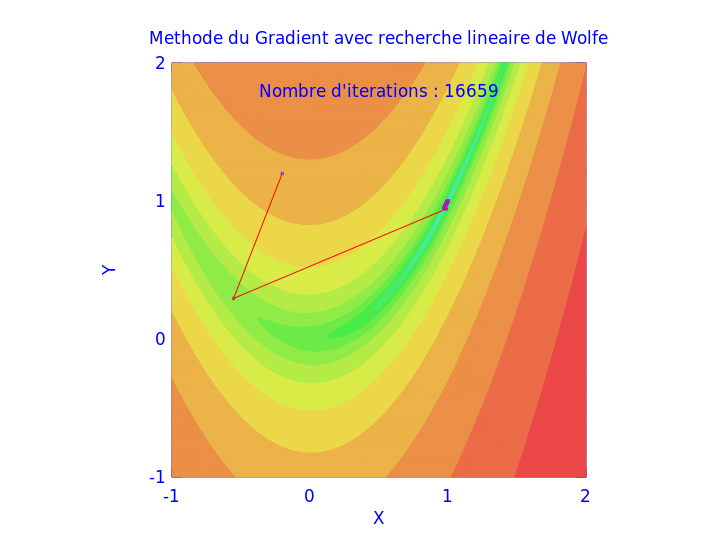
\includegraphics[width=9cm]{img/rosenbrock_gradient_wolfe.png}}
\end{figure}

On constate que l'algorithme du gradient à pas fixe converge encore très lentement en terme du nombre d'itérations, mais que l'algorithme du gradient avec Wolfe fait beaucoup moins bien qu'auparavant (même si il démarre bien en "traversant" quasiment toute la vallée d'un coup).

\begin{figure}[H]
	\centering
	\subfloat{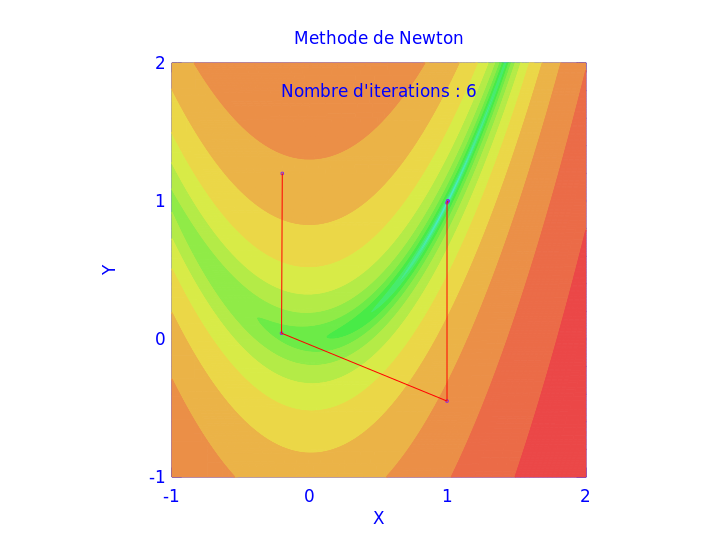
\includegraphics[width=9cm]{img/rosenbrock_newton.png}}
	\subfloat{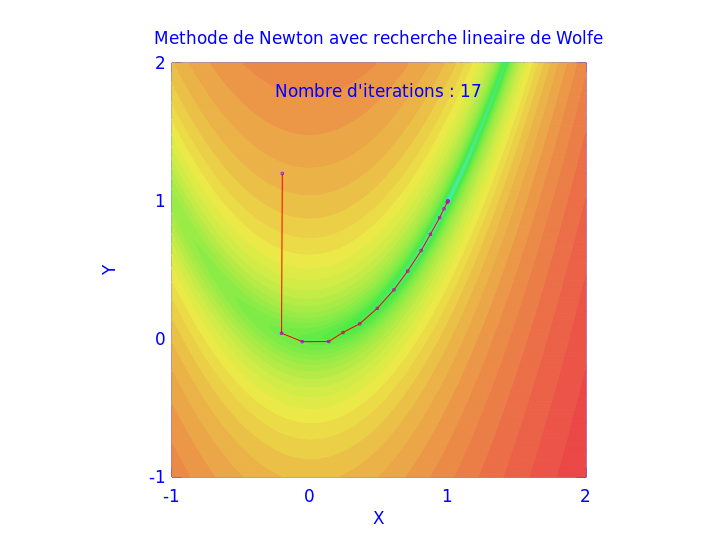
\includegraphics[width=9cm]{img/rosenbrock_newton_wolfe.png}}
\end{figure}

L'écart se creuse énormément entre les méthodes de Newton et celles du gradient. Là où les méthodes du gradient peinent à trouver le minimum en moins de quelques dizaines de millier d'itérations, les méthodes de Newton, quant à elles, convergent en seulement une dizaine. La recherche linéaire de Wolfe contraint cependant la méthode de Newton à "suivre" la vallée de Rosenbrock.

\newpage
\subsubsection{Fonction de Himmelblau}

\hspace{0.4cm}
Troisième et dernière fonction : la fonction de Himmelblau.
Elle possède 4 minimums locaux identiques 0 et un maximum local.
On prend $x_0 = (1,1)$ comme point initial pour les 3 premiers graphes puis $x_0' = (0,0)$ pour le dernier.

\begin{figure}[H]
	\centering
	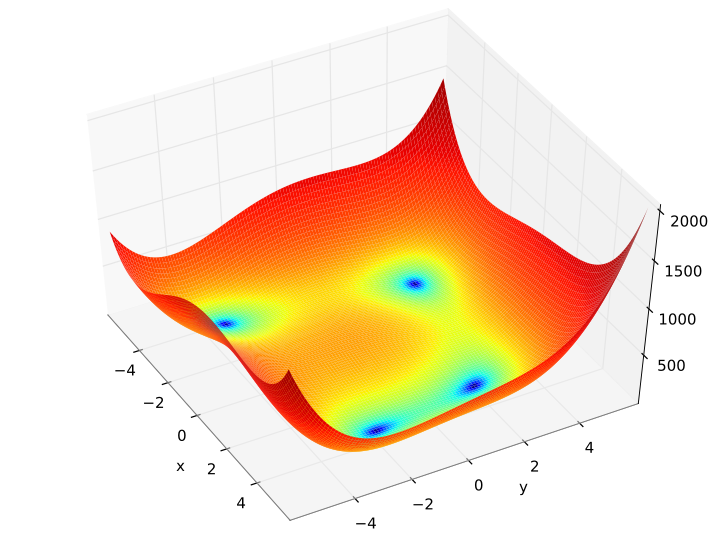
\includegraphics[width = 8cm]{img/himmelblau.png}
\end{figure}

$$
f(x,y) = (x^2 + y - 11)^2 + (x + y^2 - 7)^2
$$



\begin{figure}[h!]
	\centering
	\subfloat{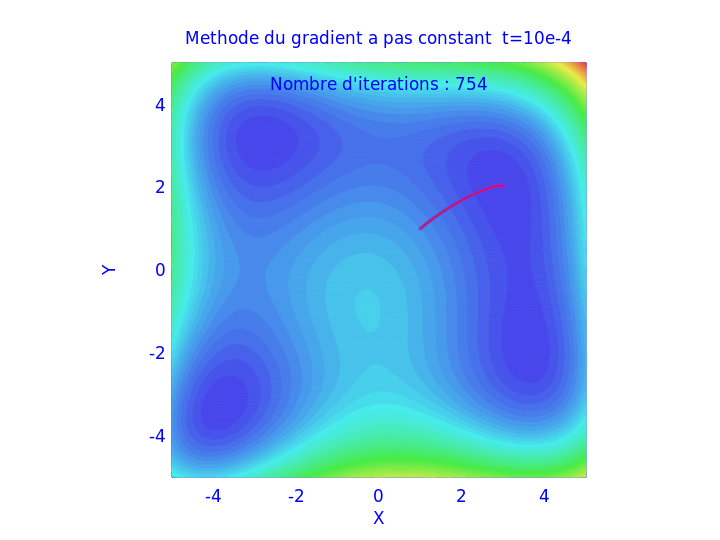
\includegraphics[width=9cm]{img/himmelblau_gradient.png}}
	\subfloat{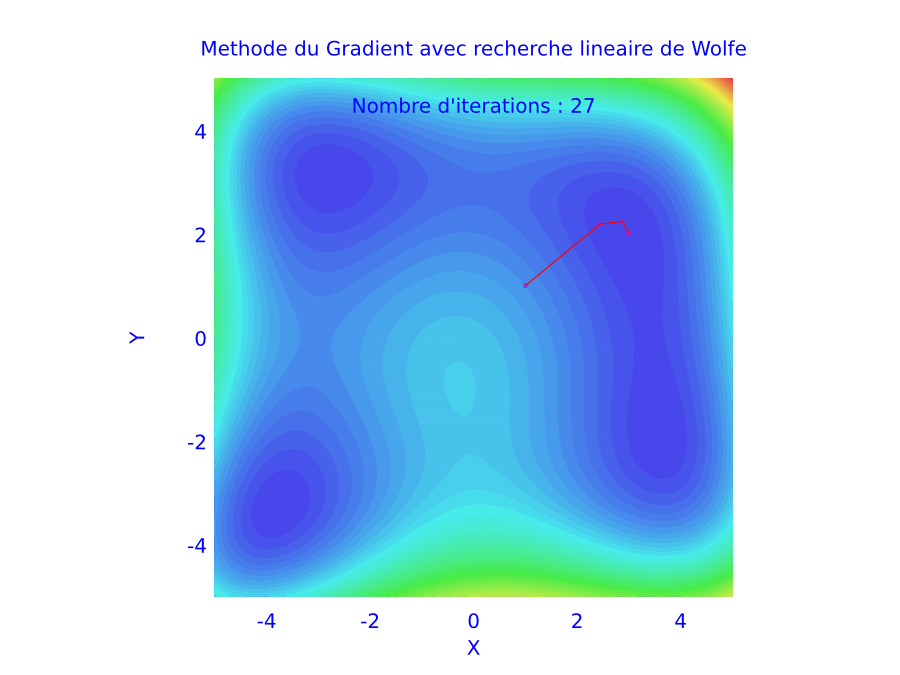
\includegraphics[width=9cm]{img/himmelblau_gradient_wolfe.png}}
\end{figure}

\begin{figure}[h!]
	\centering
	\subfloat{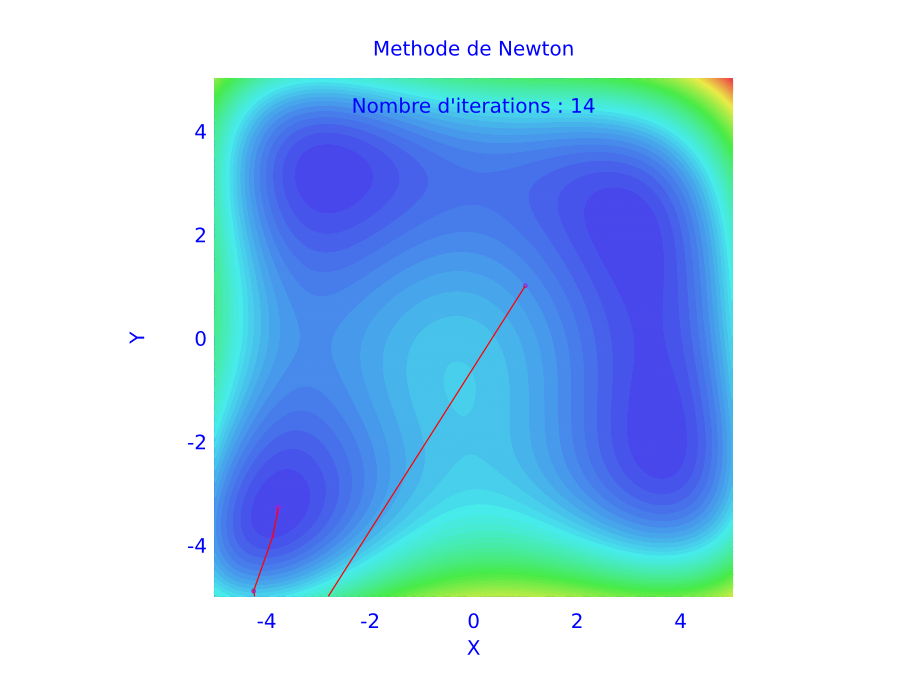
\includegraphics[width=9cm]{img/himmelblau_newton.png}}
	\subfloat{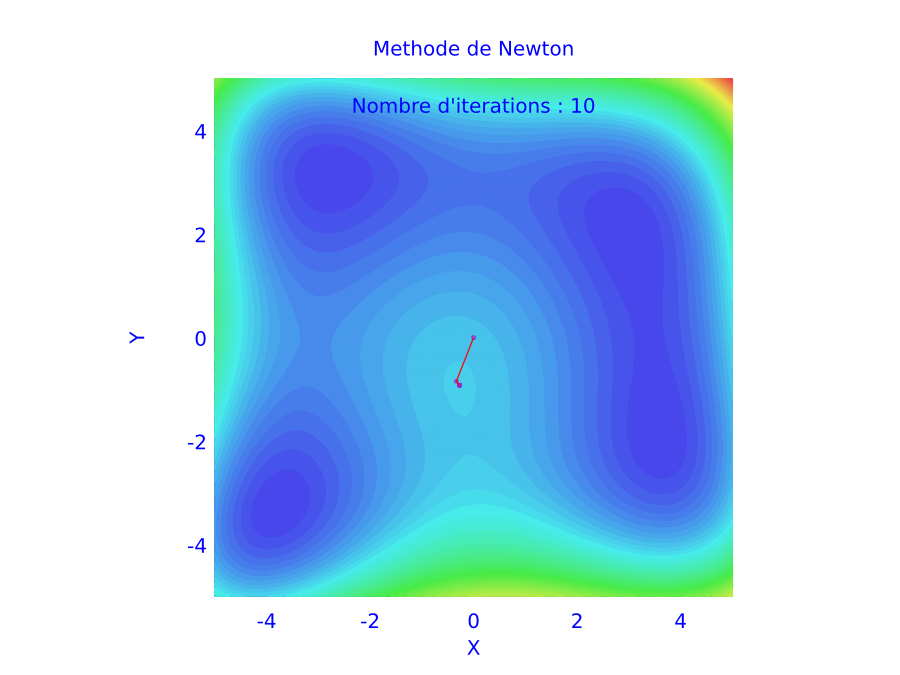
\includegraphics[width=9cm]{img/himmelblau_newton_max.png}}
\end{figure}

Les remarques faites sur la fonction de Rosenbrock sont toujours valables.
On constate que ,selon la méthode employée, on ne converge pas vers le même minimum.
De plus, comme la hessienne de cette fonction n'est pas toujours définie positive, l'algorithme de Newton peut converger vers le maximum local ou tout autre point critique. 
La recherche linéaire de Wolfe a du être adaptée car si la direction de Newton est mauvaise (direction de montée), l'algorithme ne s'arrête pas.  


\newpage
\subsection{Comparatif sur un nuage de points aléatoires}
\vspace{0.5cm}
 
 
\hspace{0.4cm}
On tire 1000 points uniformément dans le pavé $[-2,2]$x$[-2,2]$ et on lance les algorithmes sur la fonction de Rosenbrock en ces points.
On observe le nombre de convergences, le nombre d'itérations moyen et le temps d'exécution moyen dans le cas des convergences.

\subsubsection{Résultats obtenus}
\vspace{0.5cm}
\begin{tabular}{|l|c|c|c|}
  \hline
  Méthode & Nombre de convergences & Nombre d'itérations moyen & Temps d'exécution moyen (ms)\\
  \hline
  Gradient à pas constant $t = 10^{-3}$& 0 & - & - \\
  Gradient à pas constant $t = 10^{-4}$& 997 & 22953 & 13.29 \\
  Gradient avec Wolfe & 1000 & 8910 & 40.38 \\
  Newton & 1000 & 5 & 0.01 \\
  Newton avec Wolfe & 1000 & 13 & 0.03 \\
  \hline
\end{tabular}

\vspace{1cm}
La méthode du gradient avec un pas trop élevé (>$10^{-3}$) ne converge jamais. Avec un pas plus fin on arrive à une convergence correcte ($99.7\%$ ici avec un pas de $10^{-4}$), mais l'on ne peut pas prédire un bon pas avant de faire la simulation.
On voit que même si la méthode du gradient avec Wolfe fait moins d'itérations, son exécution reste environ 3 fois plus lente que la méthode du gradient à pas constant. 
Les méthodes de Newton s'exécutent beaucoup plus rapidement et l'on passe cette fois ci sous la barre de la milliseconde ce qui ne reflète pas vraiment le coùt d'une dizaine d'inversions de matrices de grande taille (on reste ici en dimension deux).

\vspace{0.5cm}
\subsubsection{Pourcentage du temps d'exécution passé dans les fonctions principales}
\vspace{0.5cm}
\begin{tabular}{|l|c|c|c|c||c|c|c||c|}
  \hline
  Méthode & multiplication & transposition & produit scalaire & inversion & valeur & gradient & hessienne & Wolfe \\
  \hline
  Gradient à pas constant & 14.7  \% & 13.8 \% & 11.9 \% & 0.0 \% & 3.27 \% & 2.59 \% & 0.0 \% & 0.0\\ 
  Gradient avec Wolfe & 17.2  \% & 22.5 \% & 17.1 \% & 0.0 \% & 3.72 \% & 4.25 \% & 0.0 \% & 21.9 \\ 
  Newton & 0.0  \% & 0.0 \% & 100.0 \% & 0.0 \% & 0.0 \% & 0.0 \% & 0.0 \% & 0.0 \\ 
  Newton avec Wolfe & 0.0  \% & 0.0 \% & 100.0 \% & 0.0 \% & 0.0 \% & 0.0 \% & 0.0 \% & 0.0 \\ 
  \hline
\end{tabular}

\vspace{1cm}
L'exécution des algorithmes de Newton est trop rapide pour pouvoir obtenir un profiling correct.
On voit cependant que les algorithmes ne sont en rien limités par les appels au simulateur mais plutôt par les opérations sur les matrices comme la multiplication ou le produit scalaire. 
La recherche linéaire de Wolfe consomme également beaucoup de ressources.

Il faudrait vérifier le comportement des algorithmes de Newton avec des matrices de plus grande taille pour vérifier l'impact sur les performances globales.



\newpage
\subsubsection{Tracé logarithmique des méthodes du gradient pour 10 points}

\vspace{0.5cm}

\hspace{0.4cm}
On trace le logarithme de la valeur de la fonction en l'itéré k pour différents points de départ.

\begin{figure}[h!]
	\centering
	\subfloat{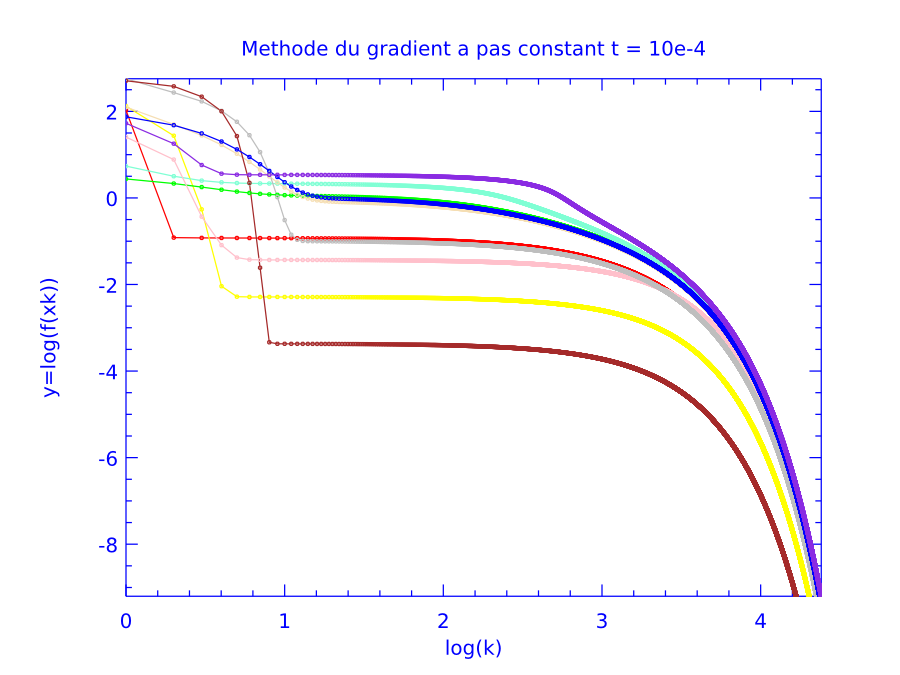
\includegraphics[width=9cm]{img/log_gradient.png}}
	\subfloat{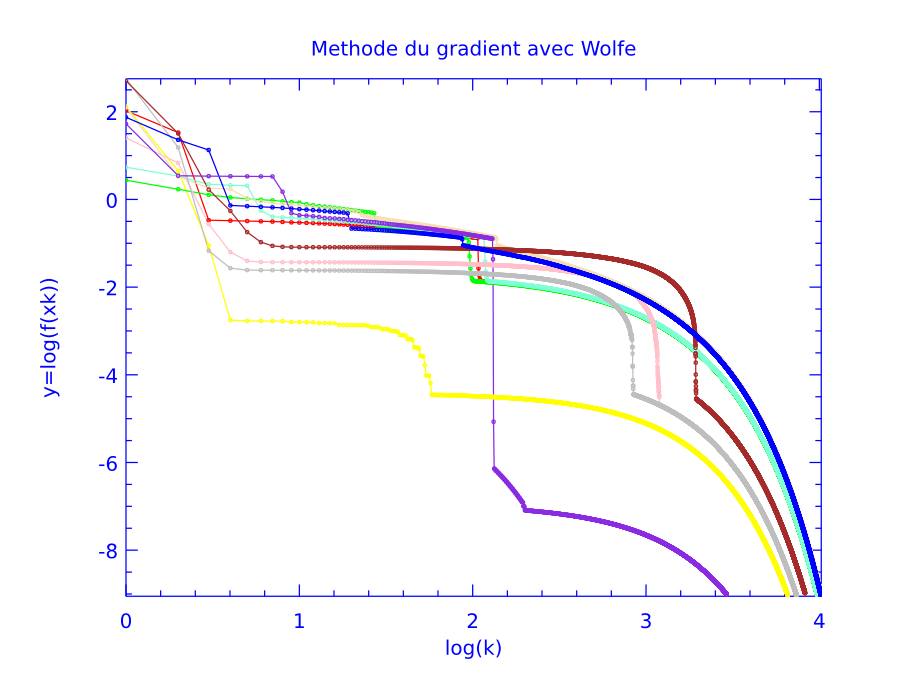
\includegraphics[width=9cm]{img/log_gradient_wolfe.png}}
\end{figure}

\vspace{0.5cm}
On voit que la recherche linéaire de Wolfe permet des sauts intéressants évitant de nombreuses itérations inutiles (la méthode du gradient seule est myope) comme constaté sur le graphique de la méthode sur la fonction de Rosenbrock.
La convergence est asymptotiquement linéaire.

\vspace{0.5cm}
\subsubsection{Tracé logarithmique des méthodes de Newton sur 10 points}

\begin{figure}[h!]
	\centering
	\subfloat{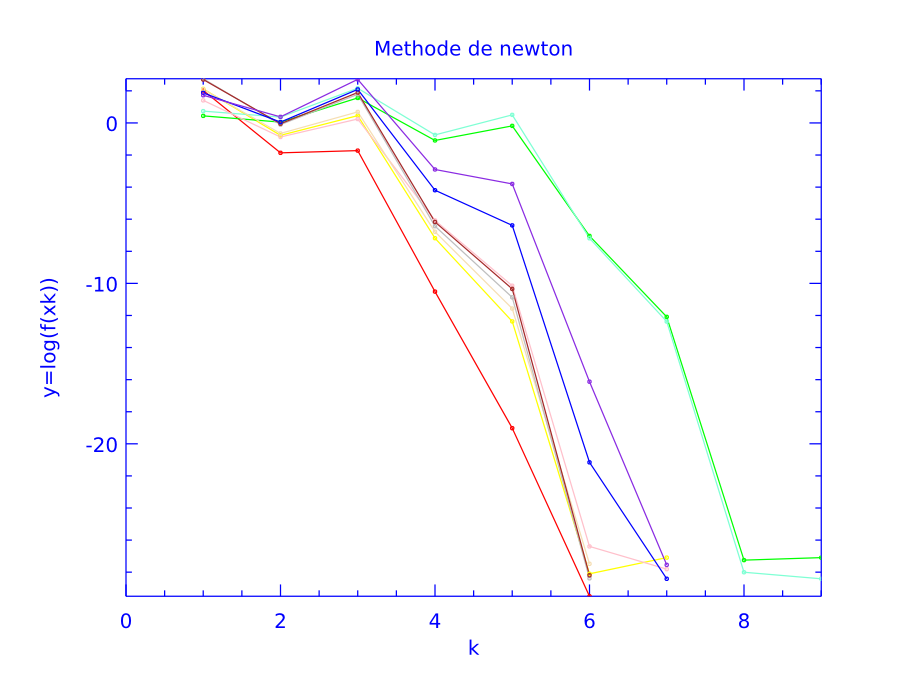
\includegraphics[width=9cm]{img/log_newton.png}}
	\subfloat{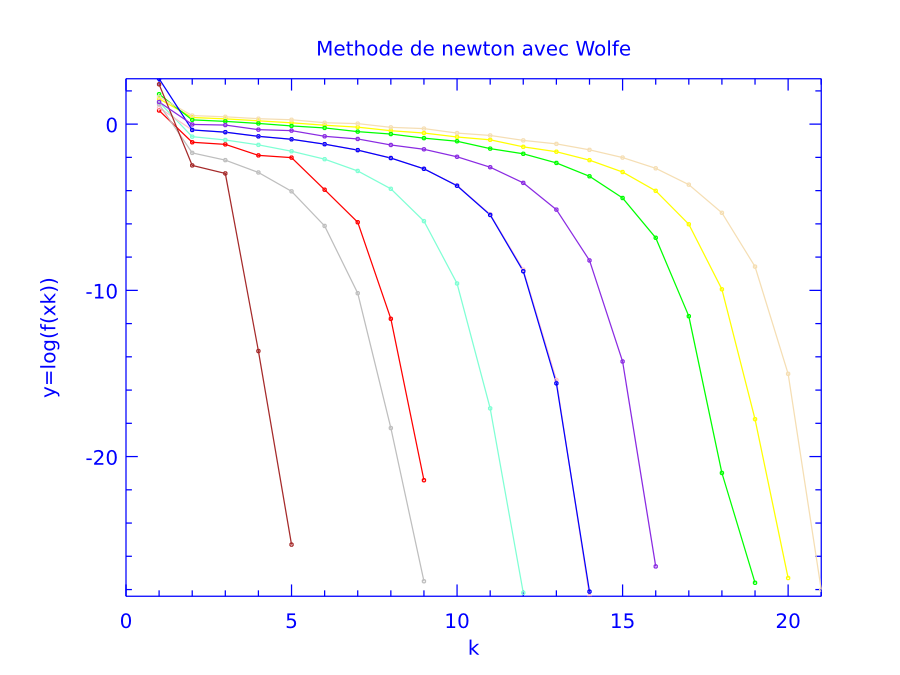
\includegraphics[width=9cm]{img/log_newton_wolfe.png}}
\end{figure}

\vspace{0.5cm}
On constate sur le premier graphe que la direction de Newton n'est pas toujours une direction de descente. 
La recherche linéaire de Wolfe tente de forcer la décroissance (ce n'est pas toujours possible) au détriment de quelques itérations en plus mais la convergence reste quadratique.

\newpage
\subsubsection{Comparaison des convergences pour un point particulier}

\begin{figure}[h!]
	\centering
	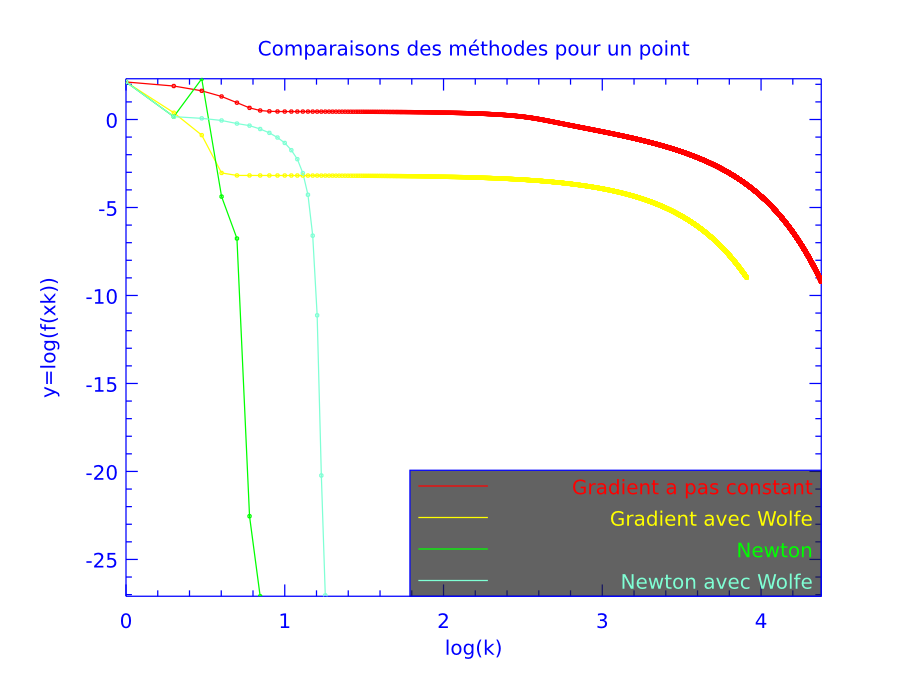
\includegraphics[width=15cm]{img/logbench.png}}
\end{figure}

\vspace{0.5cm}

La différence de convergence entre les deux types de méthode est encore plus frappante.

\vspace{1cm}
\subsection{Conclusion}
	
	\vspace{0.5cm}
	\hspace{0.4cm}
	La méthode du gradient à pas fixe est mauvaise. En plus d'être myope elle souffre d'un problème de scaling car il faut trouver le bon pas pour rendre l'algorithme convergent.	
	La recherche linéaire de Wolfe force la convergence de cet algorithme et permet en plus de sauter de nombreuses itérations inutiles.

	\vspace{0.2cm}
	La méthode BFGS couplée à Wolfe permet de se passer de la hessienne qui peut être très coûteuse à calculer puis à inverser et offre une convergence quadratique.
	
	\vspace{0.2cm}
	La méthode de Newton converge encore plus rapidemment si le cout de calcul et d'inversion n'est pas trop élevé (comme ici en dimension 2 avec une expression directe de la matrice où l'on converge en 0.1ms). Mais il ne faut pas oublier que ces méthodes ne marchent que si la hessienne est définie positive aux points de simulation, sinon on peut converger vers un point critique quelconque. Cependant, en pratique, si le point de départ est assez proche du minimum, ces méthodes convergent quand même.

	


\end{document}

